%% ====================================================================
\chapter{Model Checking}
\label{section:model:checking}
\index{Model Checking}%
\index{Verification Methods!Model Checking}%
%% ====================================================================
%
% Within the field of formal verification, 
The approach that we focus on this thesis is
\emph{model-checking}.
%% ********************************************************************
\KW{Automation}%
\index{Automation}%
%% ********************************************************************
This method will try to verify whether a model of the program
satisfies its specification.
%
%It is often called a push-button technology.
%
 
This approach was introduced by Emerson and Clarke~\cite{CE82} and by Queille and Sifakis~\cite{QS82}. The method requires a model of the system under
consideration and a property as input. The method then computes and returns either "correct" when the specification is satisfied by the program, or "incorrect" when the program does not satisfy its specification. In the case of incorrect answer, the method can explain the reason by giving a counter-example. A state in the model contains relevant information about the program. Alongside all the states of the system, the model depicts the
transitions, i.e.\ how to move from one state to another state. Every behaviour of the system is represented as a succession of transitions, starting from some initial states. States and transitions together describe the \emph{operational
  semantics}, that is, how every step of the system takes place in the model. The number of states and transitions can be finite or infinite. Model-checking aims to explore the state-space entirely from some initial states. However, when the state-space is of large size. It grows in-fact
exponentially with the number of parameters or the size of their
domain. Therefore, there have been several methods to address with the
state-space explosion problem.
%\begin{figure}[h]
%{\noindent\centering %
%  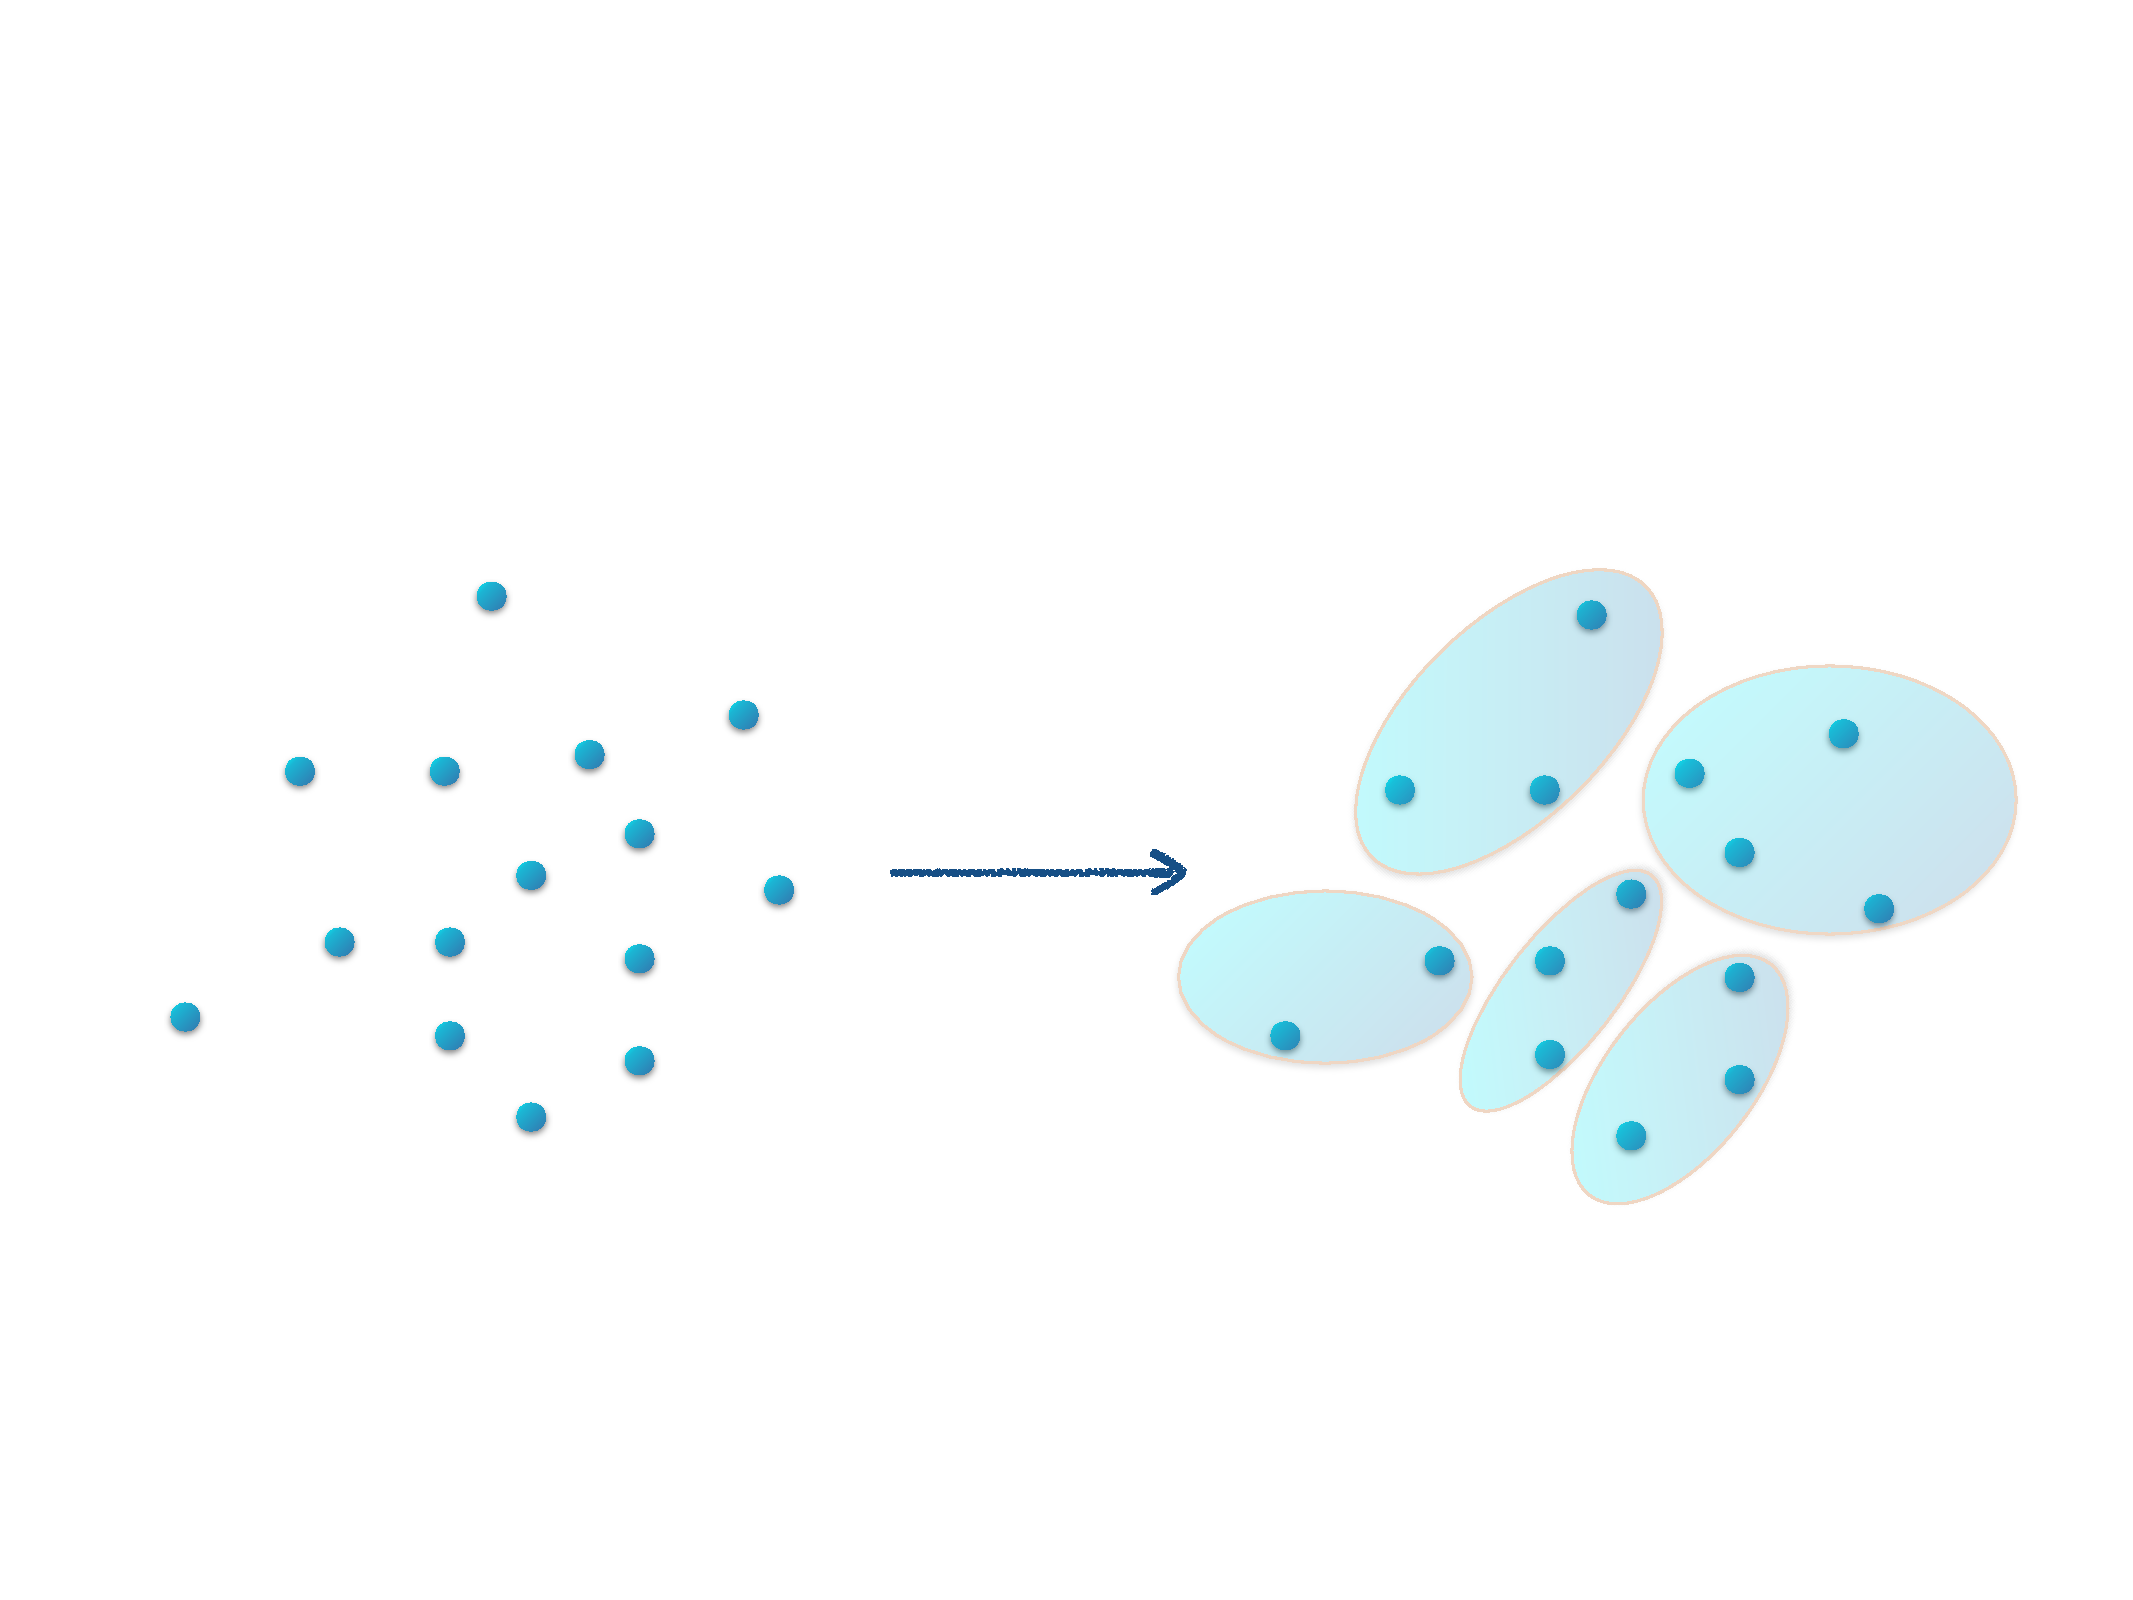
\includegraphics[trim=4cm 4cm 1.5cm 2cm,clip,scale = 0.3]{img/modelchecking.pdf}%
%  \par%
%}%
%\caption{Example of symbolic representation where the right part is a concrete reachable state-space and the left part is abstract state-space using symbolic representation}
%\label{symbolicabs}
%\end{figure}
%\vspace{1cm}
%\begin{figure}[h]
%  \centering
%  \tikzinput{img/symbolic-representations}    
%  \vspace{0.3cm}
%  \caption{Symbolic Representation}      
%\label{symbolicabs}
%\end{figure}
%\vspace{1cm}
                   
There are several techniques addressing the state-space explosion problem.
The choice of which transition to pick during the exploration can be
crucial for the efficiency of the procedure. In some cases, exploring all orderings of events is not necessary because some states can be re-visited. \emph{Partial order} techniques aim at detecting and avoiding
redundant situations, while retaining important dependencies among
actions. They however do not reduce the state-space. The main approach called \emph{symbolic
  representation}  to solve the state-space explosion problem is to avoid representing concretely all states of the system. The process is performed by designing abstract states so that each abstract state could represent a set of concrete states.  This designing process is done by \emph{dropping} irrelevant details based on properties that we want to verify. For example, consider a switch with two positions: {\tt up} and {\tt down}. The switch has a counter that indicates how many times the light was turn on. Initially, its position is {\tt down}, the light is {\tt off} and the counter is $\tt 0$. When the switch is shifted up, the light is turned on, and the counter is incremented by $\tt 1$. When we shift the switch down, the light is turned off and the counter is reset to $\tt 0$ if it had reached its maximum value. We want to verify that the switch can not be up and the light is off at the same time. If we keep all the information of the system, then, a state consists of the position of the switch, the status of the light and the value of the counter, we would have $\tt (2*2*n)$ states where $\tt n$ is the maximum value of counter. If $\tt n$ is $\tt 1000000$ then we may end up to four million states.  However, it is obvious that the counter is not needed to verify the property, so we could ignore it then a state contains only the position and status of the switch and the light denoted as $\tt [p,s]$ where $\tt p$ is the position and $\tt s$ is the state of the light. The system using the symbolic representation moves from  [{\tt down;off}]  to  [{\tt up;on}]  and conversely from  [{\tt up;on}]  to  [{\tt down;off}] . We see that the state-space exploration never visits a state that belongs to the set labeled by  [{\tt down;on}]  therefore the system is safe. The switch example is of course simple and does not reflect the complexity of today’s software. Symbolic representations are of crucial help to combat the state-space explosion, accelerate the algorithms and get them to terminate in a reasonable amount of time

%By doing that, we get an set of abstract states from reachable states of a concrete system. Thereafter, the method returns safe if the abstract states do not contain any bad state. The approach described in figure \ref{symbolicmodelchecking}.  %
%
The challenge is to find over-approximations that do not introduce
behaviours that could turn out to be bad. Indeed, the method would
return that the property is not satisfied and we would not know
whether it comes from the approximation or from the concrete system
itself. % 
                                   
%\begin{figure}
%{\noindent\centering %
%  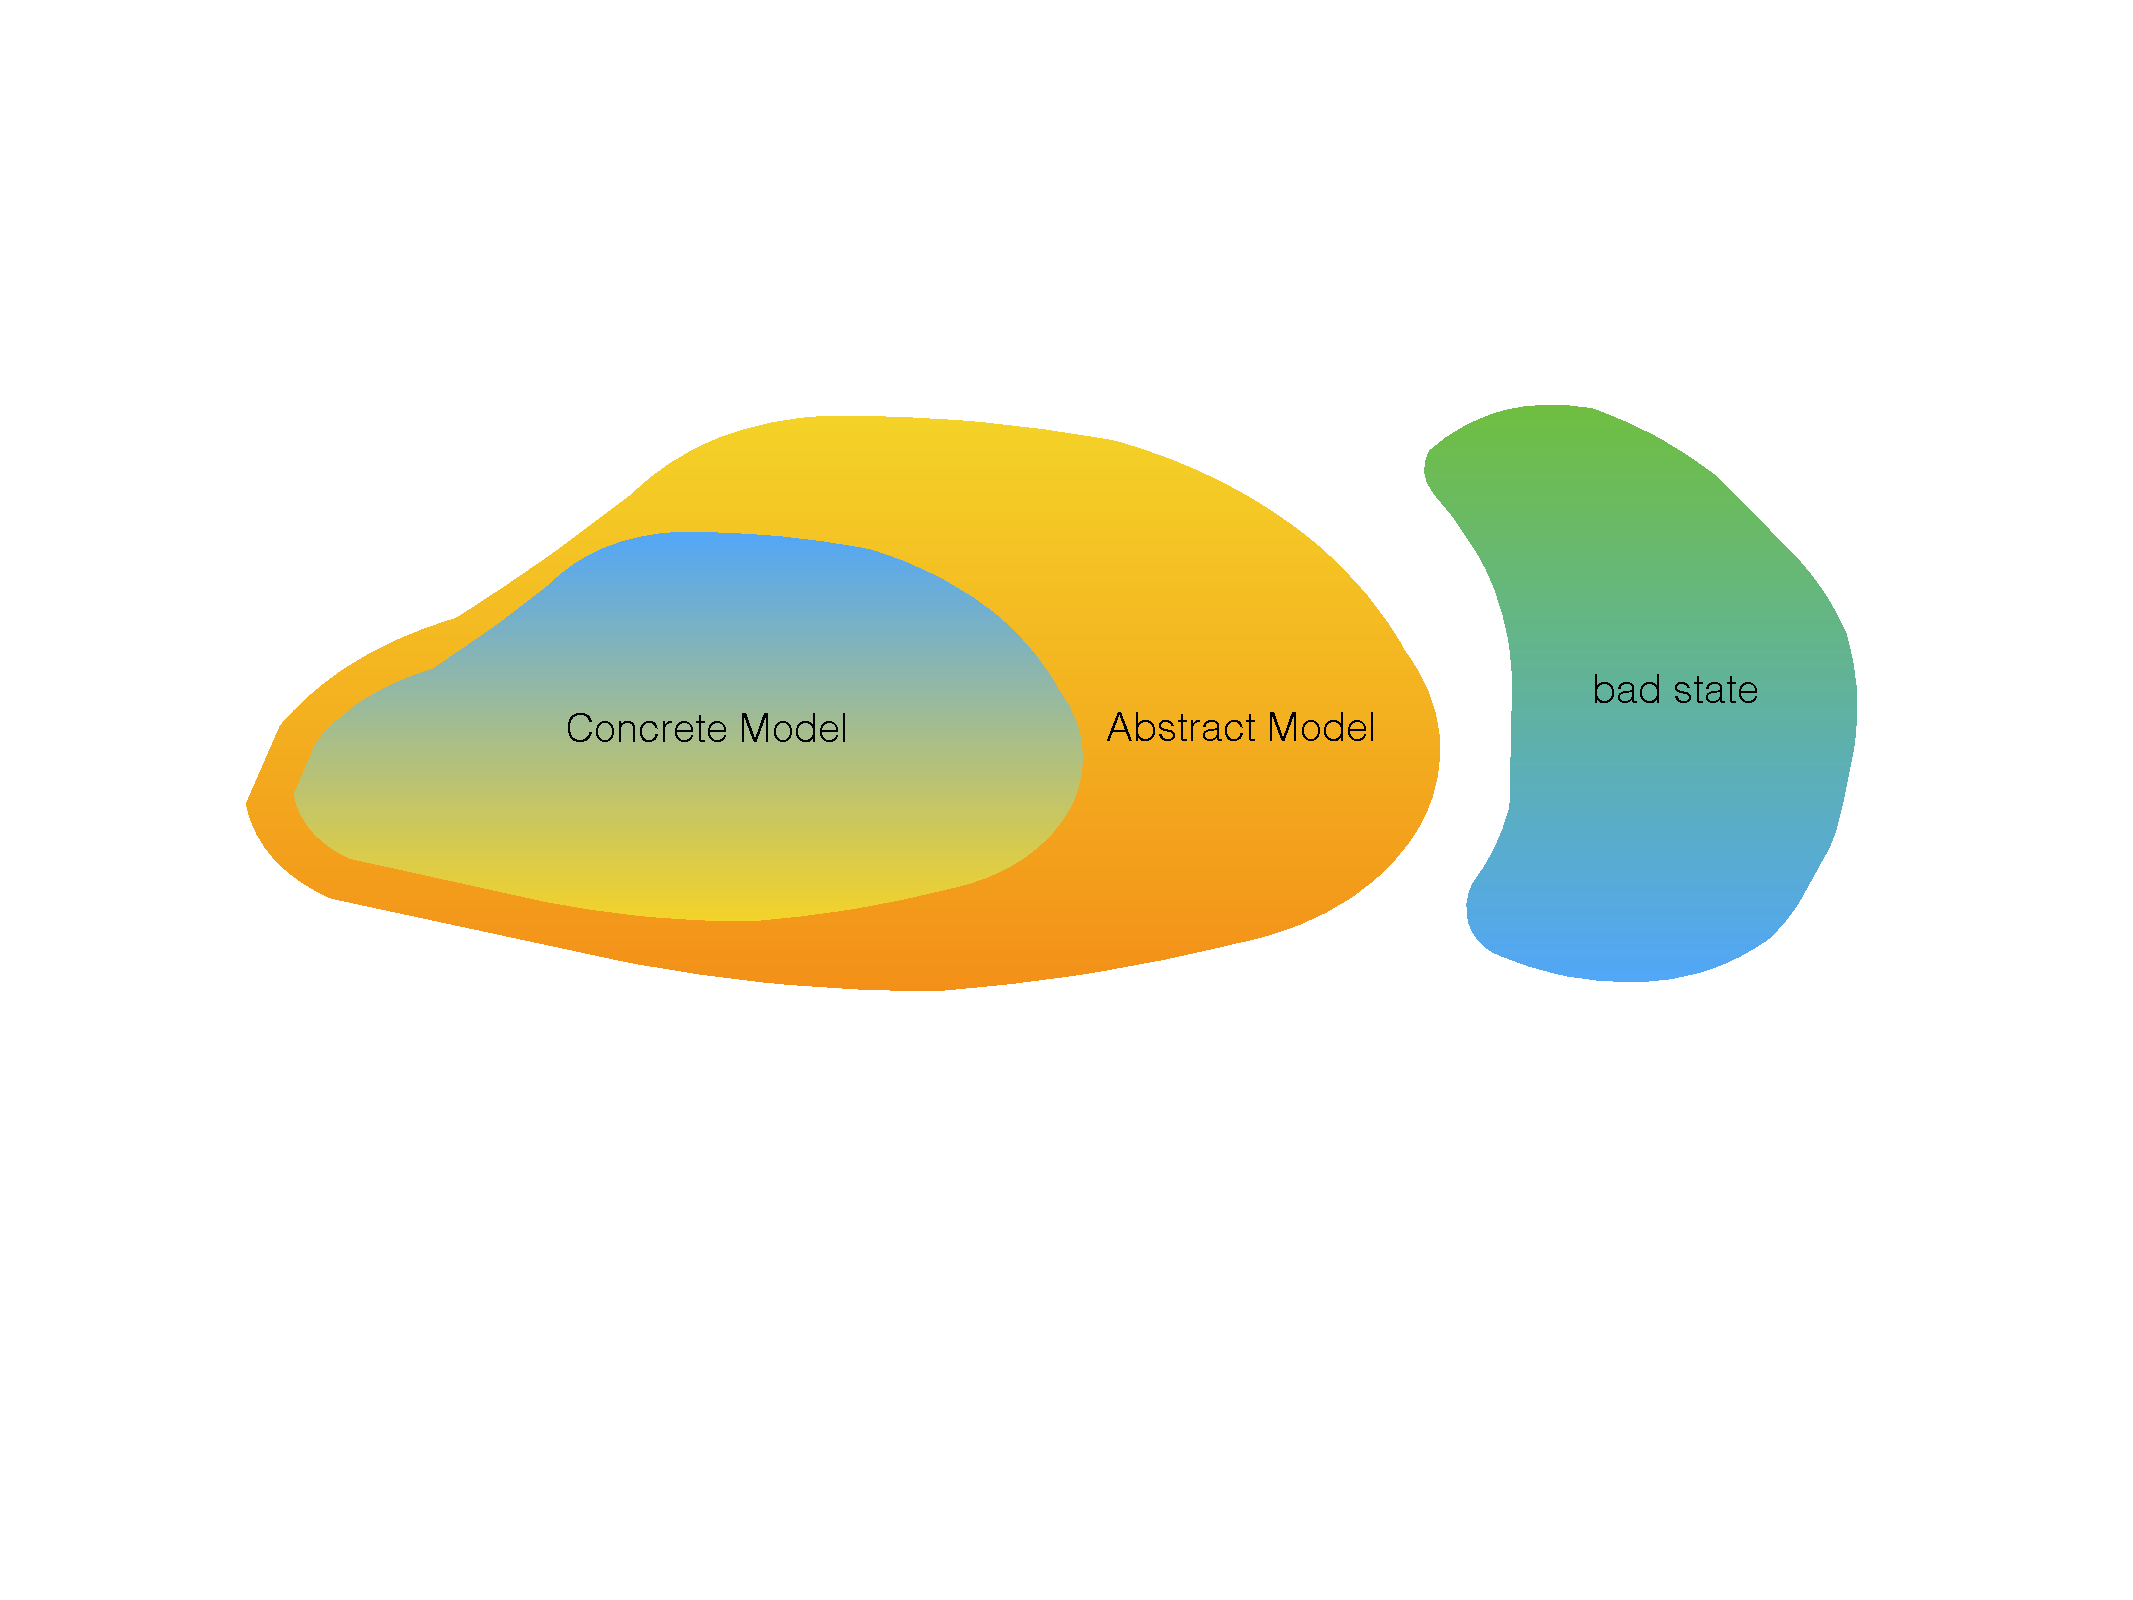
\includegraphics[trim=0cm 6cm 2cm 2cm,clip,scale = 0.25]{img/badstate.pdf}%
%  \par%
%}%
%\caption{Symbolic model checking architecture }	
%\label{symbolicmodelchecking}
%\end{figure}


%\vspace{1cm}
%\begin{figure}[h]
%  \centering
%  \tikzinput{img/approximations} 
%  \vspace{0.3cm}
%\caption{Symbolic model checking architecture }	
%\label{symbolicmodelchecking}
%\end{figure}
%\vspace{1cm}

To palliate to the imprecision caused by a too coarse
over-approximation, it is possible to analyze the returned
counter-example and find the origin of the problem. If it turns out to
be a real concrete example, the method has in fact found a bug, and
the property is surely not satisfied. Otherwise, the counter-example
comes from the approximation, that is, there is a step in the sequence
of events leading to that counter-example which is not performed by
the original system but only by the abstract model. The approximation
is be refined by discarding this step and the method should be run
anew.

Nevertheless, finding suitable over-approximations is a challenge on
its own. %
This thesis now revolves around the following problem statement.
%
%\begin{statement}
%  {\bf Safety}: %
%  {\it Given a specification and an (over-)approximation,\\does the
%    abstract system reach a bad configuration?}
%\end{statement}
%
